\documentclass[12pt, a4paper, oneside]{ctexart}
\usepackage{amsmath, amsthm, amssymb, graphicx}
\usepackage{hyperref}
\usepackage{listings}
\usepackage{xcolor}
\usepackage{color}
\usepackage{enumerate}
\usepackage{epstopdf}
\usepackage{float}
\usepackage{framed}
\usepackage[ruled,vlined]{algorithm2e}
\hypersetup{
    colorlinks=true,
    linkcolor=blue,
    filecolor=blue,      
    urlcolor=blue,
    citecolor=cyan,
}
\definecolor{dkgreen}{rgb}{0,0.6,0}
\definecolor{gray}{rgb}{0.5,0.5,0.5}
\definecolor{mauve}{rgb}{0.58,0,0.82}
\definecolor{shadecolor}{rgb}{0.5,0.5,0.5}
\lstset{ %
    language=Python,                % the language of the code
    basicstyle=\footnotesize,           % the size of the fonts that are used for the code
    numbers=left,                   % where to put the line-numbers
    %numberstyle=\tiny\color{gray},  % the style that is used for the line-numbers
    %stepnumber=2,                   % the step between two line-numbers. If it's 1, each line 
                            % will be numbered
    %numbersep=5pt,                  % how far the line-numbers are from the code
    %backgroundcolor=\color{blue},      % choose the background color. You must add \usepackage{color}
    showspaces=false,               % show spaces adding particular underscores
    %showstringspaces=false,         % underline spaces within strings
    showtabs=false,                 % show tabs within strings adding particular underscores
    frame=single,                   % adds a frame around the code
    rulecolor=\color{black},        % if not set, the frame-color may be changed on line-breaks within not-black text (e.g. commens (green here))
    tabsize=2,                      % sets default tabsize to 2 spaces
    captionpos=b,                   % sets the caption-position to bottom
    breaklines=true,                % sets automatic line breaking
    breakatwhitespace=false,        % sets if automatic breaks should only happen at whitespace
    % title=\lstname,                   % show the filename of files included with \lstinputlisting;
                            % also try caption instead of title
    keywordstyle=\color{blue},          % keyword style
    commentstyle=\color{dkgreen},       % comment style
    stringstyle=\color{mauve},         % string literal style
    escapeinside={\%*}{*)},            % if you want to add LaTeX within your code
    morekeywords={*,...}               % if you want to add more keywords to the set
}
\title{ICS\_Lab5\_Report}
\author{Xiaoma}
\date{\today}
\begin{document}
\maketitle
\section*{实验目的}
使用LC-3汇编语言实现根据输入值计算汉诺塔问题的解。
\begin{itemize}
    \item 通过中断驱动I/O键入一个字符值
    \item 判断键入字符是否为$0-9$的整数,若是则计算汉诺塔问题的解,若不是则输出相关信息
    \item 在没有键盘输入时,程序将无限循环输出学生学号
\end{itemize}
\section*{实验原理}
\subsection*{汉诺塔问题}
汉诺塔是一个数学问题,由三根杆子和许多不同直径的圆盘组成,这些圆盘可以处于任何杆子上。
问题开始时,圆盘按大小递减的顺序堆叠在一根杆上,最小的在顶部,
该问题的目标是将整个堆栈移动到最后一根杆上,移动时需遵守以下规则
\begin{itemize}
    \item 一次只能移动一个圆盘
    \item 每次移动只能取出杆上最顶部的圆盘,并将其放置于另一根杆的顶部或空杆上
    \item 任何圆盘都不能防在比其小的圆盘上面
\end{itemize}
通过计算我们可以得到汉诺塔问题的求解公式
$$H(n)=\begin{cases}
    0 \quad n = 0\\
    2H(n-1) + 1 \quad n > 0
\end{cases}$$
\begin{figure}[H]
    \centering
    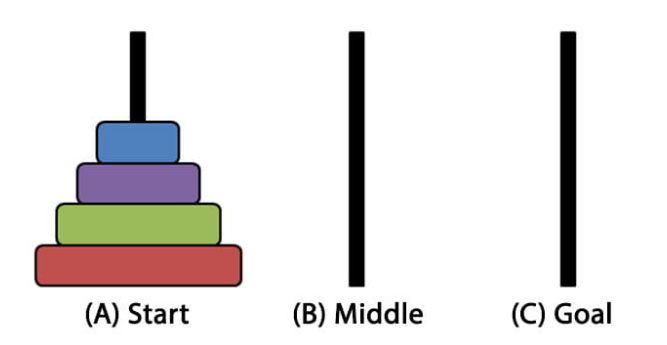
\includegraphics[scale=0.75]{3.png}
\end{figure}
\subsection*{判断键入值是否为有效值}
已知从键盘键入的值的类型为字符型,则当字符值为$0-9$时,其整型值实际为$48-57$,
故可以通过确定输入值是否在给定范围内来判断其是否为有效值,若为有效值,则中断服务程序执行
结束后,用户程序计算汉诺塔问题的解,若不是有效值,则用户程序继续循环输出学号。

\section*{实验步骤}
\subsection*{用户程序}
\subsubsection*{循环输出学号的实现}
首先使用 $.STRINGZ$ 来存放需要输出的字符串,即
\begin{lstlisting}
    StuNum .STRINGZ "PB2006xxxx\n"
\end{lstlisting}
然后使用 $.FILL$ 使用标签来存放字符串的指针,则可以使用 $trap x22$指令来输出该字符串,即 
\begin{lstlisting}
    SITESTU   .FILL StuNum
    LD R0, SITESTU
    trap x22
\end{lstlisting}
\subsubsection*{轮询键盘输入}
通过轮询键盘状态寄存器$KBSR$判断是否有键盘输入,若有则跳转至键盘中断服务程序。
\subsubsection*{求解汉诺塔问题}
采用递归的方法实现求解汉诺塔问题,根据LC-3的$JSR,RET$操作,可知寄存器$R7$保存子程序结束后返回的地址,
而如果采用递归的方式,必须使用一个栈来存储每个程序中的$R7$的值。该递归子程序的栈内容如图所示
\begin{figure}[H]
    \centering
    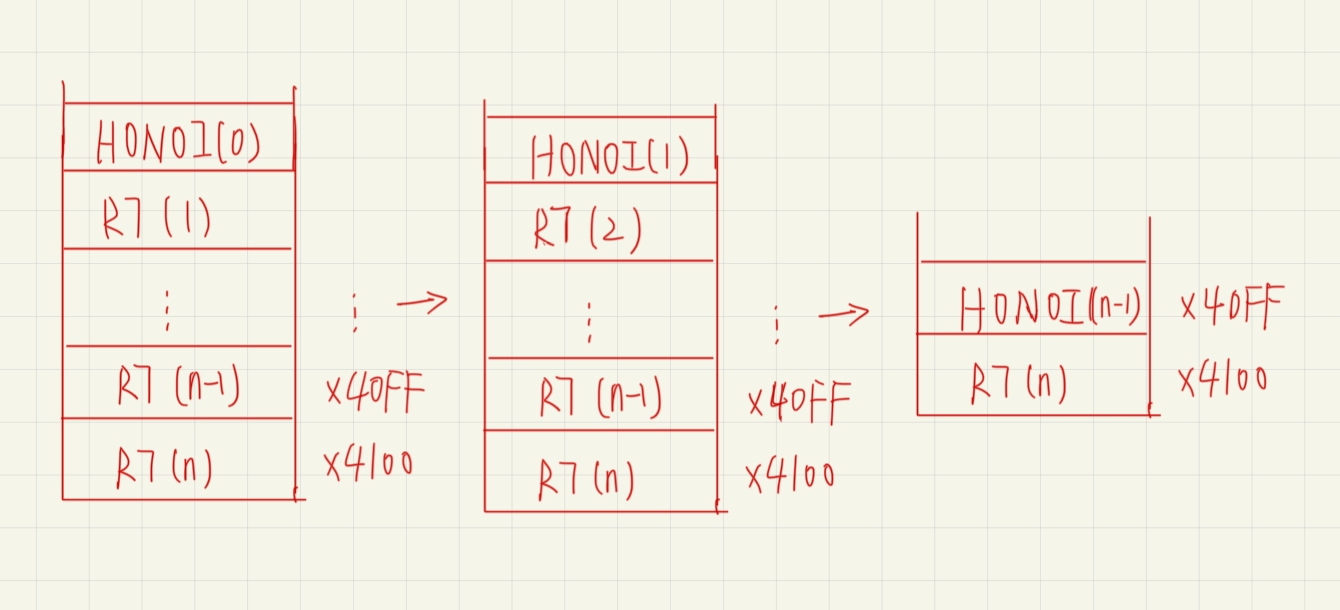
\includegraphics[scale=0.28]{1.png}
\end{figure}
当$n>0$时,进入下一级程序$HONOI(n-1)$,当下一级程序结束返回时,将结果从栈中取出,计算结果后再压入栈,返回上一级程序。
\\当$n=0$时,子程序得到结果0,并将其压入栈中,返回上一级程序。
\subsubsection*{输出答案}
若将结果直接输出到屏幕,则寄存器的值会被视为一个字符输出,故需要通过取余按位输出结果,
并且要将每一位都的值都加48,以保证输出的字符与整型值对应。
\begin{lstlisting}
L5      ADD R6, R6, #1
        LD R3, NUM2
        ADD R0, R0, R3
        BRzp L5
        LD R3, NUM3
        ADD R1, R0, R3
        ADD R6, R6, #-1
        LD R3, NUM4
        ADD R0, R6, #0
        BRz #2
        ADD R0, R0, R3
OUT1    trap x21
        ADD R0, R1, #0
        AND R6, R6, #0
L6      ADD R6, R6, #1
        ADD R0, R0, #-10
        BRzp L6
        ADD R1, R0, #10
        ADD R6, R6, #-1
        ADD R0, R6, #0
        BRz #2
        ADD R0, R0, R3
OUT2    trap x21
        ADD R0, R1, #0
        ADD R0, R0, R3
OUT3    trap x21
\end{lstlisting}
\subsection*{键盘中断服务程序}
该程序判断输入值是否为有效值的过程中同样要考虑字符型和整型的对应关系,若转化为整型后为$0-9$的整数,则输出相应信息,并存储结果。
若不是有效值,输出相应的信息。已知只有当输入值为有效值时才进行汉诺塔问题的求解,故使用一个寄存器作为判断输入是否为有效值的标志位。

\section*{实验结果}
程序运行的结果如图所示
\begin{figure}[H]
    \centering
    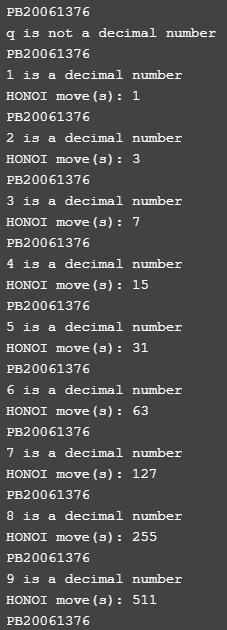
\includegraphics[scale=0.9]{2.png}
\end{figure}
\end{document}